\documentclass{article}

\usepackage{fancyhdr}
\usepackage{extramarks}
\usepackage{amsmath}
\usepackage{amsthm}
\usepackage{amsfonts}
\usepackage{tikz}
\usepackage[plain]{algorithm}
\usepackage{algpseudocode}
\usepackage{enumerate}
\usepackage{amssymb}
\usepackage{mathrsfs}
\usepackage{mathtools}
\usepackage{amsmath}
\usepackage{graphicx}

\graphicspath{ {./images} }

\usetikzlibrary{automata,positioning}

%
% Basic Document Settings
%

\topmargin=-0.45in
\evensidemargin=0in
\oddsidemargin=0in
\textwidth=6.5in
\textheight=9.0in
\headsep=0.25in

\linespread{1.1}

\pagestyle{fancy}
\lhead{\hmwkAuthorName}
\chead{\hmwkClass:\ \hmwkTitle}
\rhead{\firstxmark}
\lfoot{\lastxmark}
\cfoot{\thepage}

\renewcommand\headrulewidth{0.4pt}
\renewcommand\footrulewidth{0.4pt}

\setlength\parindent{0pt}
\setlength{\parskip}{5pt}

%
% Create Problem Sections
%

\newcommand{\enterProblemHeader}[1]{
    \nobreak\extramarks{}{Problem \arabic{#1} continued on next page\ldots}\nobreak{}
    \nobreak\extramarks{Problem \arabic{#1} (continued)}{Problem \arabic{#1} continued on next page\ldots}\nobreak{}
}

\newcommand{\exitProblemHeader}[1]{
    \nobreak\extramarks{Problem \arabic{#1} (continued)}{Problem \arabic{#1} continued on next page\ldots}\nobreak{}
    \stepcounter{#1}
    \nobreak\extramarks{Problem \arabic{#1}}{}\nobreak{}
}

\setcounter{secnumdepth}{0}
\newcounter{partCounter}
\newcounter{homeworkProblemCounter}
\setcounter{homeworkProblemCounter}{1}
\nobreak\extramarks{Problem \arabic{homeworkProblemCounter}}{}\nobreak{}

%
% Homework Problem Environment
%
% This environment takes an optional argument. When given, it will adjust the
% problem counter. This is useful for when the problems given for your
% assignment aren't sequential. See the last 3 problems of this template for an
% example.
%
\newenvironment{homeworkProblem}[1][-1]{
    \ifnum#1>0
        \setcounter{homeworkProblemCounter}{#1}
    \fi
    \section{Problem \arabic{homeworkProblemCounter}}
    \setcounter{partCounter}{1}
    \enterProblemHeader{homeworkProblemCounter}
}{
    \exitProblemHeader{homeworkProblemCounter}
}

%
% Homework Details
%   - Title
%   - Due date
%   - Class
%   - Section/Time
%   - Instructor
%   - Author
%

\newcommand{\hmwkTitle}{Homework\ \#2}
\newcommand{\hmwkDueDate}{Apr 19, 2024}
\newcommand{\hmwkClass}{MATH 140B}
\newcommand{\hmwkClassInstructor}{Professor Seward}
\newcommand{\hmwkAuthorName}{\textbf{Ray Tsai}}
\newcommand{\hmwkPID}{A16848188}

%
% Title Page
%

\title{
    \vspace{2in}
    \textmd{\textbf{\hmwkClass:\ \hmwkTitle}}\\
    \normalsize\vspace{0.1in}\small{Due\ on\ \hmwkDueDate\ at 23:59pm}\\
    \vspace{0.1in}\large{\textit{\hmwkClassInstructor}} \\
    \vspace{3in}
}

\author{
  \hmwkAuthorName \\
  \vspace{0.1in}\small\hmwkPID
}
\date{}

\renewcommand{\part}[1]{\textbf{\large Part \Alph{partCounter}}\stepcounter{partCounter}\\}

%
% Various Helper Commands
%

% define norm \norm{...}:
\DeclarePairedDelimiterX\norm[1]\lVert\rVert{{#1}}

% Useful for algorithms
\newcommand{\alg}[1]{\textsc{\bfseries \footnotesize #1}}

% For derivatives
\newcommand{\deriv}[1]{\frac{\mathrm{d}}{\mathrm{d}x} (#1)}

% For partial derivatives
\newcommand{\pderiv}[2]{\frac{\partial}{\partial #1} (#2)}

% Integral dx
\newcommand{\dx}{\mathrm{d}x}

% Probability commands: Expectation, Variance, Covariance, Bias
\newcommand{\Var}{\mathrm{Var}}
\newcommand{\Cov}{\mathrm{Cov}}
\newcommand{\Bias}{\mathrm{Bias}}
\newcommand*{\Z}{\mathbb{Z}}
\newcommand*{\Q}{\mathbb{Q}}
\newcommand*{\R}{\mathbb{R}}
\newcommand*{\C}{\mathbb{C}}
\newcommand*{\N}{\mathbb{N}}
\newcommand*{\prob}{\mathds{P}}
\newcommand*{\E}{\mathds{E}}

\begin{document}

\maketitle

\pagebreak

\begin{homeworkProblem}
  Suppose $f$ is defined in a neighborhood of $x$, and suppose $f''(x)$ exists. Show that
  \[
  \lim_{{h \to 0}} \frac{f(x + h) + f(x - h) - 2f(x)}{h^2} = f''(x).
  \]
  Show by example that the limit may exist even if $f''(x)$ does not. 

  \begin{proof}
    Put $g(h) = f(x + h) + f(x - h) - 2f(x)$. Since $g$ is differentiable in a neighborhood of $x$ and $g(h) \to 0$ as $h \to 0$, we may apply the L'Hospotal's Rule and get
    \begin{align*}
      \lim_{{h \to 0}} \frac{g(h)}{h^2} 
      &= \lim_{{h \to 0}} \frac{f'(x + h) - f'(x - h)}{2h} \\
      &= \lim_{{h \to 0}} \frac{f'(x + h) - f'(x)}{2h} - \lim_{{h \to 0}} \frac{f'(x - h) - f'(x)}{2h} \\
      &= \lim_{{h \to 0}} \frac{f'(x + h) - f'(x)}{2h} - \lim_{{k \to 0}} \frac{f'(x + k) - f'(x)}{-2k} \\
      &= \frac{f''(x)}{2} + \frac{f''(x)}{2} = f''(x).
    \end{align*}

    Consider $f(x) = \begin{cases} 1 & x > 0 \\
      0 & x = 0 \\
      -1 & x < 0 \end{cases}$. $f$ is not continuous at $0$, so $f''(0)$ does not exist. But then $f(h) + f(-h) - 2f(0) = 0$ for all $h > 0$, so $\lim_{{h \to 0}} \frac{f(x + h) + f(x - h) - 2f(x)}{h^2}$ exists.
  \end{proof}
\end{homeworkProblem}

\newpage

\begin{homeworkProblem}
  Suppose $a \in \mathbb{R}^1$, $f$ is a twice-differentiable real function on $(a, \infty)$, and $M_0$, $M_1$, $M_2$ are the least upper bounds of $|f(x)|$, $|f'(x)|$, $|f''(x)|$, respectively, on $(a, \infty)$. Prove that
  \begin{gather}
    M_1^2 \leq 4M_0M_2.
  \end{gather}
  Does $M_1^2 \leq 4M_0M_2$ hold for vector-valued functions too?

  \begin{proof}
    Let $x \in (a, \infty)$. Put $h > 0$. By Taylor's Theorem, there eixsts $t \in (x, x + 2h)$ such that
    \[
      f(x + 2h) = f(x) + 2hf'(x) + 2h^2f''(t),
    \]
    that is,
    \[
      f'(x) = \frac{1}{2h}[f(x + 2h) - f(x)] + hf''(t).
    \]
    But then
    \[
      -\frac{M_0}{h} - hM_2 \leq f'(x) \leq \frac{M_0}{h} + hM_2.
    \]
    It follows that
    \[
      M_1^2 \leq \left(\frac{M_0}{h} + hM_2\right)^2 = \left(\frac{M_0^2}{h^2} + h^2M_2^2\right) + 2M_0M_2 \leq 4M_0M_2,
    \]
    as $\frac{M_0^2}{h^2} + h^2M_2^2 \geq 2M_0M_2$ by AM-GM.

    To show that $M_1^2 = 4M_0M_2$ can actually happen, take $a = -1$, define
    \[
      f(x) = 
      \begin{cases} 
        2x^2 - 1 & x \in (-1, 0)\\
        \frac{x^2 - 1}{x^2 + 1} & x \in [0, \infty)
      \end{cases}.
    \] 
    we know
    \[
      f'(x) = 
      \begin{cases} 
        4x & x \in (-1, 0) \\
        \frac{4x}{(x^2 + 1)^2} & x \in [0, \infty)
      \end{cases}, \  f''(x) = 
      \begin{cases} 
        4 & x \in (-1, 0) \\
        \frac{4(-3x^2 + 1)}{(x^2 + 1)^3} & x \in [0, \infty)
      \end{cases}, \  f'''(x) = 
      \begin{cases} 
        0 & x \in (-1, 0) \\
        \frac{48x(x^2 - 1)}{(x^2 + 1)^4} & x \in [0, \infty)
      \end{cases}
    \]
    Since $f' < 0$ when $x < 0$ but $f' > 0$ when $x > 0$, $f(x)$ monotonically decreases from 1 to $-1$ then monotonically approaches $1$, and thus $M_0 = 1$. 

    When $x < 0$, since $f'' > 0$, $f'$ monotonically increases from $-4$ to 0. Notice that $\frac{4(-3x^2 + 1)}{(x^2 + 1)^3} = 0$ has a single positive root at $x = \frac{1}{\sqrt{3}}$. Since $f'(0) = 0$, $f'(1/\sqrt{3}) = \frac{3\sqrt{3}}{4}$, and $\lim_{x \to \infty} f'(x) = 0$, $|f'(x)| \leq \frac{3\sqrt{3}}{4} < 4$ for nonnegative $x$. Hence, $M_1 = 4$.
    
    Notice that $f'''(x) = 0$ has a single positive root at $x = 1$. But then $f''(0) = 4, f''(1) = -1, \lim_{x \to \infty} f''(x) = 0$, so $M_2 = 4$.

    Therefore, the equality of (1) holds for this example.

    We now show that (1) also holds for vector valued functions. Let $f'(x) = (f_1(x), \dots, f_n(x))$ be a twice differentiable vector valued function on $(a, \infty)$. Let $M_0^f$, $M_1^f$, $M_2^f$ be the least upper bounds of $\norm{f(x)}$, $\norm{f'(x)}$, $\norm{f''(x)}$, respectively. Pick $\epsilon > 0$. There exists $c \in (a, \infty)$ such that $\norm{f'(c)} \geq M_1^f - \epsilon$. Let $u = \frac{f'(c)}{\norm{f'(c)}}$ and define $g(x) = u \cdot f(x)$. Let $M_0^g$, $M_1^g$, $M_2^g$ be the least upper bounds of $|g(x)|$, $|g'(x)|$, $|g''(x)|$, respectively. We know 
    \[
      M_1^g \geq g'(c) = u \cdot f'(c) = \norm{f'(c)} \geq M_1^f - \epsilon,
    \]
    for arbitrary $\epsilon$, and thus $M_1^g \geq M_1^f$. But then by Cauchy-Schwarz inequality, 
    \[
      g(x)^2 \leq \norm{u}\norm{f(x)}^2 \leq M_0, \quad g'(x)^2 \leq \norm{u}\norm{f''(x)}^2 \leq M_2,
    \]
    as $\norm{u} = 1$. Hence, applying (1) on $g$, we get $M_1^f \leq M_1^g \leq 2\sqrt{M_0^gM_2^g} \leq 2\sqrt{M_0^fM_2^f}$.
  \end{proof}
\end{homeworkProblem}

\newpage

\begin{homeworkProblem}
  Suppose $f$ is a real function on $(-\infty, \infty)$. Call $x$ a fixed point of $f$ if $f(x) = x$.

  \begin{enumerate}[(a)]
    \item If $f$ is differentiable and $f'(t) \neq 1$ for every real $t$, prove that $f$ has at most one fixed point.
    \begin{proof}
      Suppose for contradiction that $f$ has multiple fixed points, say $x, y$, $x < y$. By MVT, there exists $t \in (x, y)$ such that
      \[
        f(y) - f(x) = x - y = (x - y)f'(t).
      \]
      But then $f'(t) = 1$, contradiction.
    \end{proof}
    \item Show that the function $f$ defined by
    \[
      f(t) = t + (1 + e^t)^{-1}
    \]
    has no fixed point, although $0 < f'(t) < 1$ for all real $t$.
    \begin{proof}
      We can easily see that
      \[
        f'(t) = 1 + \frac{-e^t}{(1 + e^t)^2}.
      \]
      Since $e^t, (1 + e^t)^2 > 0$ and $e^t < (1 + e^t)^2$, we have $0 < \frac{e^t}{(1 + e^t)^2} < 1$, and so $0 < f'(t) < 1$.

      Suppose $t$ is a fixed point of $f$, which implies $t + (1 + e^t)^{-1} = t$. But then $(1 + e^t)^{-1} = 0$, contradiction. 
    \end{proof}
    \item However, if there is a constant $A < 1$ such that $|f'(t)| \leq A$ for all real $t$, prove that a fixed point of $f$ exists, and that $x = \lim_{n \to \infty} x_n$, where $x_1$ is an arbitrary real number and
    \[
      x_{n+1} = f(x_n)
    \]
    for $n = 1, 2, 3, \ldots$.
    \begin{proof}
      Since $x_{n + 1} = f(x_n)$ and $x_n = f(x_{n - 1})$, by MVT,
      \[
        |f(x_n) - f(x_{n - 1})| = |x_{n + 1} - x_n| = |f'(t)(x_{n} - x_{n - 1})| \leq |f'(t)||(x_{n} - x_{n - 1})| \leq A|x_{n} - x_{n - 1}|,
      \]
      for some $t$, and thus $|x_{n + 1} - x_n| \leq A^{n - 1}|x_2 - x_1|$. But then for $m, n \geq N$, 
      \begin{align*}
        |x_m - x_n| 
        &\leq |x_m - x_{m - 1}| + \dots + |x_{n + 1} - x_n| \\
        &= (x_2 - x_1)\sum_{k = n - 1}^{m - 2} A_k \\
        &\leq (x_2 - x_1)\sum_{k = N}^{\infty} A_k \leq \frac{|x_2 - x_1|A^N}{1 - A}.
      \end{align*}
      As $A < 1$, $|x_m - x_n| \to 0$ as $N \to \infty$. Therefore, $(x_n)$ is a Cauchy sequence in the reals, which converges to some $x$. But then $f(x) = \lim\limits_{n \to \infty} f(x_n) = x_{n + 1} = x$, so $x$ is a fixed point.
    \end{proof}

    \break 

    \item Show that the process described in (c) can be visualized by the zig-zag path
    \[
      (x_1, x_2) \to (x_2, x_2) \to (x_2, x_3) \to (x_3, x_3) \to (x_3, x_4) \to \ldots .
    \]
    \begin{proof}
      Take $f(x) = \frac{1 - x}{2}$ and consider the following diagram:
      \begin{center}
        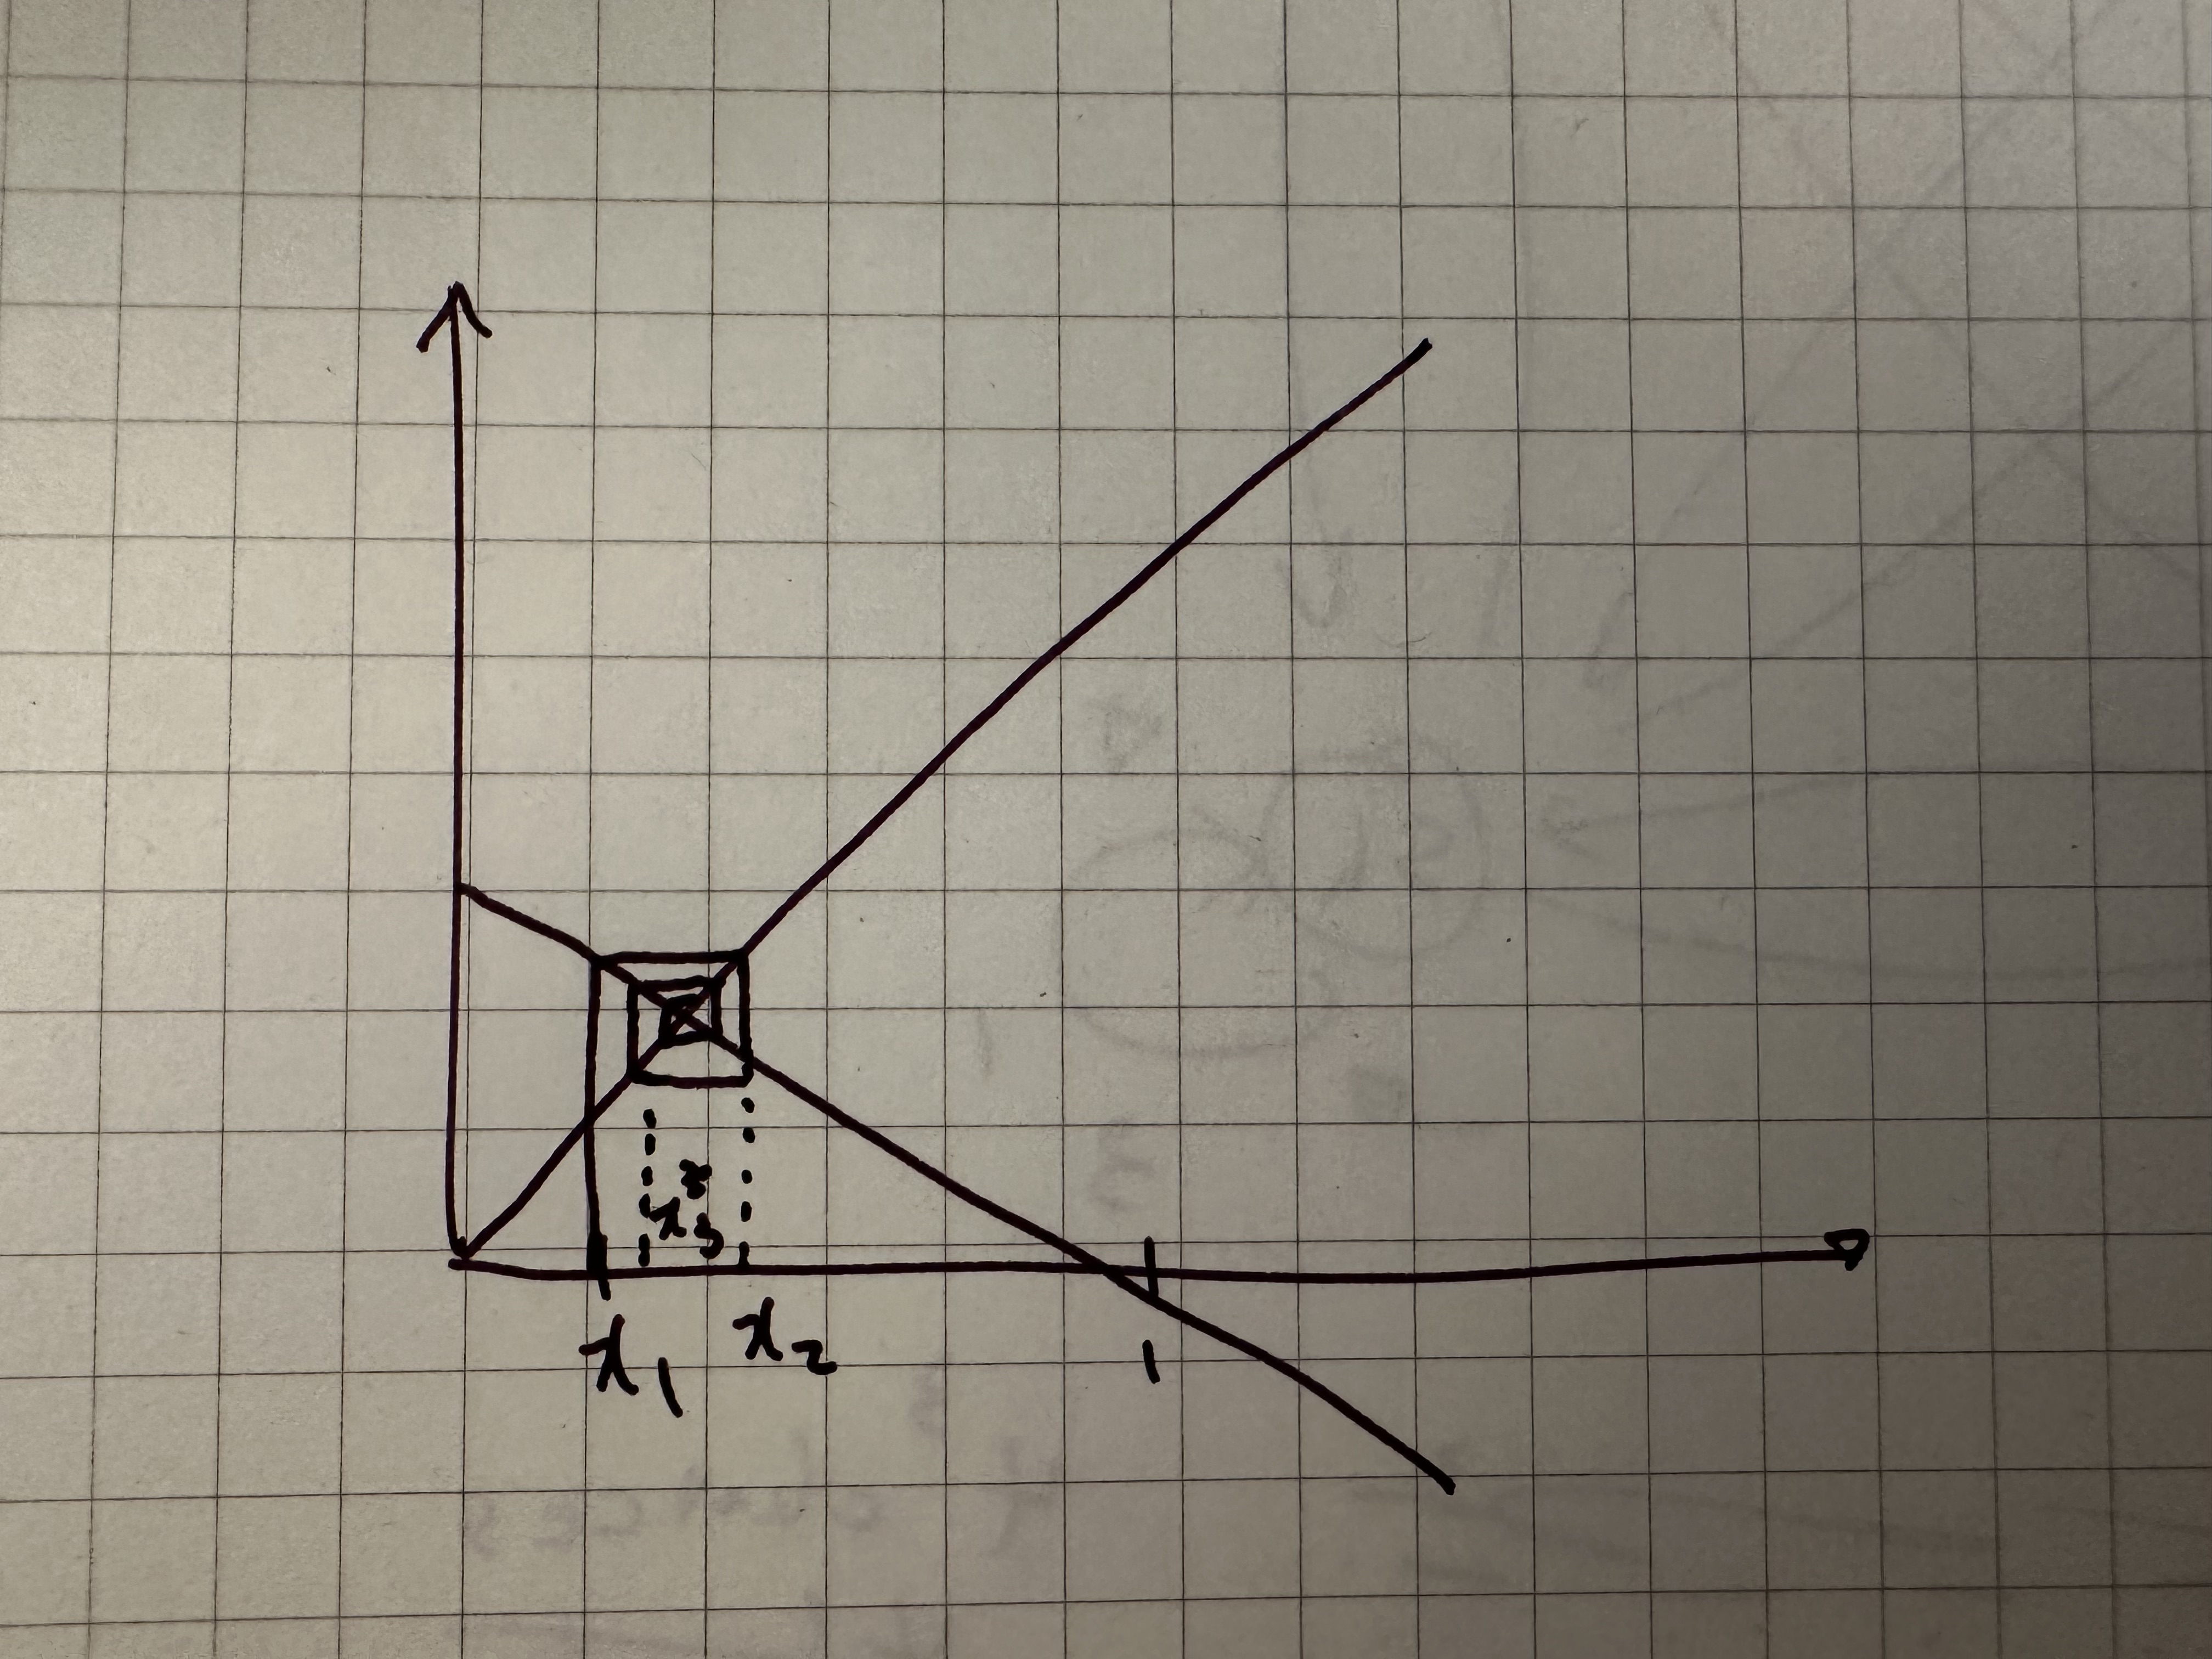
\includegraphics[width=0.8\textwidth]{Q4d}
      \end{center}
    \end{proof}
  \end{enumerate}
\end{homeworkProblem}

\newpage

\begin{homeworkProblem}
  Suppose $\alpha$ increases on $[a, b]$, $a \leq x_0 \leq b$, $\alpha$ is continuous at $x_0$, $f(x_0) = 1$, and $f(x) = 0$ if $x \neq x_0$. Prove that $f \in \mathscr{R}(\alpha)$ and that $\int f \, d\alpha = 0$.

  \begin{proof}
    Pick arbitrary $\epsilon > 0$. We first note that the infimum of $f(x)$ over any interval in $[a, b]$ is 0, so $L(P, f, \alpha) = 0$. Since $\alpha$ is continuous at $x_0$, there exists $\delta > 0$ such that $|\alpha(x) - \alpha(x_0)| < \epsilon/2$ whenever $|x - x_0| < \delta$. Consider the partition $P = \{a, x_0 - \delta', x_0 + \delta', b\}$, where $0 < \delta' < \min \{\delta, x_0 - a, b - x_0\}$. We then have
    \begin{align*}
      U(P, f, \alpha)
      &= \alpha(x_0 + \delta') - \alpha(x_0 - \delta') \\
      &= (\alpha(x_0 + \delta') - \alpha(x_0)) + (\alpha(x_0) - \alpha(x_0 - \delta')) \\
      &< \frac{\epsilon}{2} + \frac{\epsilon}{2} = \epsilon.
    \end{align*}
    Hence, $U(P, f, \alpha) - L(P, f, \alpha) = \epsilon$, and so $f \in \mathscr{R}(\alpha)$ by Theorem 6.6. Since $L(P, f, \alpha) \leq \int f d\alpha \leq U(P, f, \alpha)$, we have $\int f d\alpha = 0$. 
  \end{proof}
\end{homeworkProblem}

\newpage

\begin{homeworkProblem}
  Suppose $f \geq 0$, $f$ is continuous on $[a, b]$, and $\int_a^b f(x) \, dx = 0$. Prove that $f(x) = 0$ for all $x \in [a, b]$.

  \begin{proof}
    Suppose for the sake of contradicion that there exists some $x_0 \in [a, b]$ with $f(x_0) = \epsilon$, for some $\epsilon > 0$. Since $f$ is continuous, there exists $\delta > 0$ such that $|f(x) - f(x_0)| < \epsilon$ for all $|x - x_0| < \delta$. Consider the partition $P = \{a, x_0 - \delta', x_0 + \delta', b\}$, where $0 < \delta' < \min \{\delta, x_0 - a, b - x_0\}$. We know $m = \inf f(x) > 0$, for $x \in (x_0 - \delta', x_0 + \delta')$. But then $L(P, f) \geq 2\delta'm > 0$, which forces $ \underline{\int}_a^b f(x) dx > 0$, contradiction.
  \end{proof}
\end{homeworkProblem}

\newpage

\begin{homeworkProblem}
  Define three functions $\beta_1, \beta_2, \beta_3$ as follows: $\beta_j(x) = 0$ if $x < 0$, $\beta_j(x) = 1$ if $x > 0$ for $j = 1, 2, 3$; and $\beta_1(0) = 0$, $\beta_2(0) = 1$, $\beta_3(0) = 1/2$. Let $f$ be a bounded function on $[-1, 1]$.

  \begin{enumerate}[(a)]
    \item Prove that $f \in \mathscr{R}(\beta_1)$ if and only if $f(0+)$ equals $f(0)$ and that then
    \[
      \int f \, d\beta_1 = f(0).
    \]
    \begin{proof}
      Suppose $f \in \mathscr{R}(\beta_1)$. Pick $\epsilon > 0$. There exists partition $P$ such that 
      \[
        U(P, f, \beta_1) - L(P, f, \beta_1) < \epsilon.
      \]
      Let $P^*$ be a refinement which contains 0. Let $\delta \in P^*$ such that $[0, \delta]$ is an interval given by the partition $P$. Then, $U(P^*, f, \beta_1) - L(P^*, f, \beta_1) = \sup f(x) - \inf f(x) < \epsilon$, $x \in [0, \delta]$. But then, $|f(t) - f(0)| < \epsilon$ whenever $t \in (0, \delta)$. Hence, $f(0+) = f(0)$.

      We now suppose $f(0+) = f(0)$. Pick $\epsilon > 0$. There exists $\delta > 0$ such that $|f(t) - f(0)| < \epsilon/2$ whenever $t \in (0, \delta)$. Let $\delta' < \min(1, \delta)$ be positive. Consider the partition $P = \{-1, 0, \delta', 1\}$. Then,
      \[
        U(P, f, \beta_1) - L(P, f, \beta_1) = f(s) - f(t) \leq |f(s) - f(0)| + |f(t) - f(0)| < \epsilon,
      \]
      for some $s, t \in [0, \delta']$. Hence, by Theorem 6.6, $f \in \mathscr{R}(\beta_1)$. Note that for any $P$ which contains $0$, we have $U(P, f, \beta_1) = M$ and $L(P, f, \beta_1) = m$, where $M = \sup_{x \in (0, \delta')} f(x)$ and $m = \inf_{x \in (0, \delta')} f(x)$. But then $M < f(0) + \epsilon$ and $m > f(0) - \epsilon$. Hence,
      \[
        f(0) - \epsilon < L(P, f, \beta_1) \leq \int f \, d\beta_1 \leq U(P, f, \beta_1) < f(0) + \epsilon,
      \]
      for arbitrary $\epsilon$, and the result follows.
    \end{proof}
    \item State and prove a similar result for $\beta_2$.
    \begin{proof}
      We show that $f \in \mathscr{R}(\beta_2)$ if and only if $f(0-)$ equals $f(0)$ and that then $\int f \, d\beta_2 = f(0)$.
      
      Suppose $f \in \mathscr{R}(\beta_2)$. Pick $\epsilon > 0$. There exists partition $P$ such that 
      \[
        U(P, f, \beta_2) - L(P, f, \beta_2) < \epsilon.
      \]
      Let $P^*$ be a refinement which contains 0. Let $-\delta \in P^*$ such that $[-\delta, 0]$ is an interval given by the partition $P$. Then, $U(P^*, f, \beta_2) - L(P^*, f, \beta_2) = \sup f(x) - \inf f(x) < \epsilon$, $x \in [-\delta, 0]$. But then, $|f(t) - f(0)| < \epsilon$ whenever $t \in (-\delta, 0)$. Hence, $f(0-) = f(0)$.

      We now suppose $f(0-) = f(0)$. Pick $\epsilon > 0$. There exists $\delta > 0$ such that $|f(t) - f(0)| < \epsilon/2$ whenever $t \in (-\delta, 0)$. Let $\delta' < \min(1, \delta)$ be positive. Consider the partition $P = \{-1, -\delta', 0, 1\}$. Then,
      \[
        U(P, f, \beta_2) - L(P, f, \beta_2) = f(s) - f(t) \leq |f(s) - f(0)| + |f(t) - f(0)| < \epsilon,
      \]
      for some $s, t \in [0, \delta']$. Hence, by Theorem 6.6, $f \in \mathscr{R}(\beta_2)$. Note that for any $P$ which contains $0$, we have $U(P, f, \beta_2) = M$ and $L(P, f, \beta_2) = m$, where $M = \sup_{x \in (\delta', 0)} f(x)$ and $m = \inf_{x \in (\delta', 0)} f(x)$. But then $M < f(0) + \epsilon$ and $m > f(0) - \epsilon$. Hence,
      \[
        f(0) - \epsilon < L(P, f, \beta_2) \leq \int f \, d\beta_2 \leq U(P, f, \beta_2) < f(0) + \epsilon,
      \]
      for arbitrary $\epsilon$, and the result follows.
    \end{proof}

    \break

    \item Prove that $f \in \mathscr{R}(\beta_3)$ if and only if $f$ is continuous at $0$.
    \begin{proof}
      Suppose $f \in \mathscr{R}(\beta_3)$. Pick $\epsilon > 0$. There exists partition $P$ such that 
      \[
        U(P, f, \beta_3) - L(P, f, \beta_3) < \epsilon.
      \]
      Let $P^*$ be a refinement which contains 0. Let $[x_i, 0]$, $[0, x_{i + 1}]$ be the intervals given by $P^*$ which contains $0$. Then, 
      \[
        U(P^*, f, \beta_3) - L(P^*, f, \beta_3) = \frac{1}{2}\left(\sup_{x \in [x_i, 0]} f(x) - \inf_{x \in [x_i, 0]} f(x) + \sup_{x \in [0, x_{i + 1}]} f(x) - \inf_{x \in [0, x_{i + 1}]} f(x)\right) < \epsilon/2
      \]
      But then, $|f(t) - f(0)| < \epsilon$ whenever $t \in (-\delta, \delta)$, where $\delta = \min(|x_i|, |x_{i + 1}|)$. Hence, $f$ is continuous at $0$. 

      We now suppose $f$ is continuous at $0$. Pick $\epsilon > 0$. There exists $\delta > 0$ such that $|f(t) - f(0)| < \epsilon/2$ whenever $t \in (-\delta, \delta)$. Let $\delta' < \min(1, \delta)$ be positive. Consider the partition $P = \{-1, -\delta', \delta', 1\}$. Then,
      \[
        U(P, f, \beta_3) - L(P, f, \beta_3) = f(s) - f(t) \leq |f(s) - f(0)| + |f(t) - f(0)| < \epsilon,
      \]
      for some $s, t \in [-\delta', \delta']$. Hence, by Theorem 6.6, $f \in \mathscr{R}(\beta_2)$.
    \end{proof}
    \item If $f$ is continuous at $0$ prove that
    \[
      \int f \, d\beta_1 = \int f \, d\beta_2 = \int f \, d\beta_3 = f(0).
    \]
    \begin{proof}
      We have already shown $\int f \, d\beta_1 = \int f \, d\beta_2 = f(0)$, from (a), (b). It remains show $\int f \, d\beta_3 = f(0)$.

      Pick $\epsilon > 0$. There exists $\delta > 0$ such that $|f(t) - f(0)| < \epsilon/2$ whenever $|t| < \delta$. But then for any $P$ which contains $-\delta, 0,\delta$, we have $U(P, f, \beta_3) < f(0) + \epsilon$ and $L(P, f, \beta_3) > f(0) - \epsilon$. Hence, 
      \[
        f(0) - \epsilon < L(P, f, \beta_3) \leq \int f \, d\beta_3 \leq U(P, f, \beta_3) < f(0) + \epsilon,
      \]
      for arbitrary $\epsilon$, and the result follows.
    \end{proof}
  \end{enumerate}
\end{homeworkProblem}

\newpage

\begin{homeworkProblem}
  If $f(x) = 0$ for all irrational $x$, $f(x) = 1$ for all rational $x$, prove that $f \notin \mathscr{R}$ on $[a, b]$ for any $a < b$.

  \begin{proof}
    Take any partition $P = \{x_0 = a, \dots, x_n = b\}$. Notice that there exists an irrational in any interval, so $L(P, f) = 0$. But then $\Q$ is dense in $\R$, so for any distinct $x_i, x_{i + 1}$, there exists $q \in \Q$ such that $x_i < q < x_{i + 1}$. But then $U(P, f) = \sum_{i = 1}^n (x_i - x_{i - 1}) = b - a > 0$. Hence, $\inf U(P, f) = b - a \neq 0 = \sup L(P, f)$, and the result now follows.
  \end{proof}
\end{homeworkProblem}
\end{document}